\documentclass[conference]{IEEEtran}

% ========= 日本語対応(LuaLaTeX推奨) =========
\usepackage{luatexja}
\usepackage{luatexja-fontspec}
\setmainjfont{HaranoAjiMincho}
\setsansjfont{HaranoAjiGothic}

% ========= 一般パッケージ =========
\usepackage{amsmath,amssymb}
\usepackage{graphicx}
\usepackage{booktabs}
\usepackage{array}
\usepackage{url}
\usepackage[hidelinks]{hyperref}
\usepackage{cite}
\usepackage{siunitx}
\sisetup{
  detect-all = true,
  per-mode   = symbol,
  range-phrase = --,
  product-units = single
}
\let\meter\metre

% ========= 図・グラフ =========
\usepackage{tikz}
\usetikzlibrary{arrows.meta,decorations.pathreplacing,calc,patterns}
\usepackage{pgfplots}
\pgfplotsset{compat=1.18}

% \usepackage{subcaption}  % ← 使わない
\usepackage[caption=false,font=footnotesize]{subfig}

% ========= タイトル =========
\title{セイコーエプソン酒田Fab 8インチライン立ち上げ\\
DRAM技術導入から量産化そしてその役割(1997--2001)}

\author{%
  \IEEEauthorblockN{三溝 真一 (Shinichi Samizo)}%
  \IEEEauthorblockA{独立系半導体研究者(元セイコーエプソン)\\%
  Independent Semiconductor Researcher (ex-Seiko Epson)\\%
  Email: \href{mailto:shin3t72@gmail.com}{shin3t72@gmail.com}\\%
  GitHub: \url{https://github.com/Samizo-AITL}}%
}

\begin{document}
\maketitle

\begin{abstract}
\textbf{(日本語)}\\
本稿は,1997--2001年にセイコーエプソン酒田事業所が
三菱電機からの技術移管により
\SI{0.5}{\micro\meter} $\rightarrow$ \SI{0.35}{\micro\meter} $\rightarrow$ \SI{0.25}{\micro\meter}
のDRAMプロセスを短期間で立ち上げ,量産化した過程を整理する。
主眼はDRAM導入・量産化であり,Pause/Disturb Refresh不良の解析と対策,歩留まり推移,
および\emph{量産インフラとしての役割}を明確化する。
その後,社内設計によるVSRAM開発やNANYA 0.18\,$\mu$m評価を経て,
DRAMの役割を終えた後に,酒田Fabが社内外のロジック/高耐圧混載CMOS展開に
寄与した戦略的意義を振り返る。\\[0.7ex]

\textbf{(English)}\\
This paper documents the introduction and mass production of DRAM processes
(\SI{0.5}{\micro\meter} $\rightarrow$ \SI{0.35}{\micro\meter} $\rightarrow$ \SI{0.25}{\micro\meter})
transferred to Seiko Epson's Sakata Fab (1997--2001).
We focus on DRAM-specific failure analyses (Pause/Disturb Refresh), countermeasures, and yield evolution,
clarifying the DRAM line's role as manufacturing infrastructure.
Later, VSRAM development and evaluation of a NANYA 0.18\,$\mu$m process marked the end of memory products,
while the acquired process infrastructure supported Epson's strategies in logic, SoC, and high-voltage mixed-CMOS.
\end{abstract}

\begin{IEEEkeywords}
DRAM, VSRAM/PSRAM, \SI{0.25}{\micro\meter} process, retention failure, disturb failure, Sakata Fab, technology transfer, SCF
\end{IEEEkeywords}

\section{序論}
1997年,当時の半導体産業は \textit{Windows 95} の世界的普及や
Intel Pentium II の登場を背景に急成長局面にあった。
パソコンの性能向上と普及拡大が同時に進み,
メモリ容量・処理性能に対する市場要求は急速に高まっていた。

製造技術面では,8インチウェーハラインの整備と
\SI{0.35}{\micro\meter} 世代プロセスへの移行が加速し,
DRAMおよびロジックLSI分野における国際競争が激化していた。

セイコーエプソンは山形県酒田市に新設した 8インチFabにおいて,
三菱電機からの技術移管を通じて
\SI{0.5}{\micro\meter} $\rightarrow$ \SI{0.35}{\micro\meter} $\rightarrow$ \SI{0.25}{\micro\meter}
の三世代DRAMプロセスを短期間で習得し量産化に至った。

本稿では,このDRAM技術導入と量産化の過程を主軸として,
Pause/Disturb Refresh不良の解析と対策,歩留まり推移を整理する。
さらに,酒田FabのDRAM量産ラインが,
その後のロジック/高耐圧混載CMOS開発の\emph{インフラ}として果たした役割を振り返る。

\section{第1章:\texorpdfstring{\SI{0.5}{\micro\meter}}{0.5µm} と 
\texorpdfstring{\SI{0.35}{\micro\meter}}{0.35µm} 世代の立ち上げ}

\subsection{\SI{0.5}{\micro\meter} 16M DRAM:三菱移管による順調な立ち上げ}
酒田Fabの最初の量産は \SI{0.5}{\micro\meter} 世代16M DRAMであった。
三菱電機・熊本Fabで確立された装置仕様・処理条件を移管し,
大きな問題もなく短期間で量産に到達した。
この成功により,酒田Fabは「新規立ち上げFabとして量産能力を有する」ことを実証した。

\begin{itemize}
  \item 熊本Fabの実績プロセスを装置・処理条件ごとに導入
  \item 初期歩留まりから安定して高水準を維持
  \item 酒田Fabが本格的量産拠点として機能することを確立
\end{itemize}

\subsection{\SI{0.35}{\micro\meter} 64M DRAM:洗浄フロー差異と層間ばらつきの顕在化}
筆者はこの \SI{0.35}{\micro\meter} 世代から酒田Fabの立ち上げに参画した。  
この世代では,酒田Fab独自の洗浄フローが致命的な問題を引き起こした。

\subsubsection*{初期の困難}
試作ロットではSEM観察すら困難なパターン崩壊が多発。
熊本Fabでは安定していた条件が再現できず,
立ち上げは停滞した。

\subsubsection*{原因解析}
徹底調査の結果,熊本と酒田で\textbf{洗浄フローが異なる}ことが判明した。
\begin{itemize}
  \item 熊本:硫酸過水 $\rightarrow$ アンモニア過水 $\rightarrow$ 塩酸過水(3段)
  \item 酒田:アンモニア過水 $\rightarrow$ 塩酸過水(前段の硫酸過水を省略)
\end{itemize}

硫酸過水は有機残渣を強力に除去し,酸化膜表面をクリーンに保つ前処理である。
これを省略した酒田フローでは,
表面に微量の有機汚染や残渣が残留し,
後段のプラズマ処理と干渉して
局所的な膜厚ばらつきや異常エッチングを誘発した。
その結果,\textbf{層間膜のばらつきとパターン形状崩壊}が顕在化した。

0.5µm世代では寸法マージンが広く問題化しなかったが,
0.35µm世代では微細化により
「硫酸過水の有無が形状形成の可否を決定する」ことが明確となった。

\subsubsection*{解決策:完全「鏡写し」}
最終解決は熊本Fabのフローを一切省略せず,
\textbf{洗浄を含めて完全に鏡写しで導入する}ことであった。
これにより不良は解消し,量産移行に成功した。

\subsection{小括}
\begin{itemize}
  \item \SI{0.5}{\micro\meter} 世代:三菱移管により順調に立ち上げ。
  \item \SI{0.35}{\micro\meter} 世代:硫酸過水を省略した洗浄フロー差異が致命傷となり,
        層間膜ばらつき・形状崩壊を引き起こした。
  \item 教訓:\textbf{プロセス移管は洗浄工程を含め「完全鏡写し」が必須}である。
  \item 筆者は \SI{0.35}{\micro\meter} 世代立ち上げから参画し,
        本課題解析と対策実施に直接関与した。
\end{itemize}

\section{第2章:\texorpdfstring{\SI{0.25}{\micro\meter}}{0.25µm} 世代64M DRAMの立ち上げ}

\subsection{プロセス概要}
\SI{0.25}{\micro\meter} 世代では,初めて KrF エキシマレーザステッパを本格導入し,
従来の i線リソグラフィから一気に波長短縮が図られた。
この「0.25µm世代=KrF世代」への移行により,
微細化と同時にリーク電流制御やキャパシタ高容量化の新技術が必須となった。

プロセスの主要仕様を Table~\ref{tab:process25} に示す。

\begin{table}[h]
\centering
\caption{\SI{0.25}{\micro\meter} 64M DRAM プロセス概要}
\label{tab:process25}
\begin{tabular}{|p{3.2cm}|p{4.8cm}|}
\hline
\textbf{項目 / Item} & \textbf{内容 / Description} \\
\hline
\textbf{電源電圧 / Supply Voltage} & 2.5V(メモリセル・周辺・I/O) \newline *2.5V for Memory Cell, Peripheral, and I/O* \\
\hline
\textbf{セルキャパシタ構造 / Cell Capacitor Structure} & スタック型キャパシタ \newline *Stacked capacitor structure* \\
\hline
\textbf{ウェル構成 / Well Structure} & メモリセルにトリプルウェル構造を採用 \newline *Triple-well adopted in memory cell region* \\
\hline
\textbf{ワードライン構造 / Word Line} & デバイデッドWL構造,WSA-ALA接続 \newline *Divided word-line structure with WSA-ALA connection* \\
\hline
\textbf{ビットライン形成 / Bit Line} & WSB-CVDにより,BLとBLコンタクトを同時形成 \newline *Bit line and bit line contact formed simultaneously by WSB-CVD* \\
\hline
\textbf{ストレージノード処理 / Storage Node Surface Treatment} & 粗面化処理により容量値1.5~1.8倍向上 \newline *Surface roughening improved capacitance by 1.5–1.8×* \\
\hline
\end{tabular}
\end{table}

\noindent
このように,0.25µm世代は単なる寸法微細化に留まらず,
\begin{itemize}
  \item 低電圧化(2.5V駆動)
  \item キャパシタ容量確保のための粗面化処理
  \item トリプルウェル導入によるセル耐性向上
  \item 新規材料(WSB-CVD)の採用によるビットライン形成
\end{itemize}
といった,多角的なプロセス革新が同時に進められた。

\subsection{SCF方式と初期歩留まり}
1998年,酒田Fabは \SI{0.25}{\micro\meter} 世代64M DRAMの立ち上げを開始した。
ここで採用されたのが \emph{Short Cycle Feedback (SCF)} 方式である。
SCF方式とは,各要素技術に定められたマニュアル規格を短期間で満足するよう,
暫定処理条件を一次確定していく方式である。

筆者はこの \SI{0.25}{\micro\meter} 世代立ち上げの最初から参画し,
量産化および量産対応までを一貫して担当した。

立ち上げフローは以下の通りであった:
\begin{enumerate}
  \item 熊本Fabから受領した処理条件を各要素技術へ展開
  \item SCFにより,各要素技術ごとに暫定処理条件を一次確定
  \item 電子流動票へ処理条件と品質規格を反映
  \item 形状ロットを流動させ,各工程でSEM測長・断面観察を実施し,所望形状を確認
  \item QAロットを投入し,歩留まりおよび信頼性試験で条件を検証
  \item 信頼性確認後,量産条件を確定し,量産へ移行
\end{enumerate}

この結果,初期歩留まり65\%という極めて高い値を達成した。
従来,新世代DRAMの初期歩留まりは20--30\%程度が一般的であり,
酒田Fabは大幅に上回る成果を示した。

\subsection{保持時間モデルと不良モード解析}
不良は主に \emph{Pause Refresh Fail} に集中した。  
リフレッシュを停止しセル保持を確認する試験で,
32ms $\rightarrow$ 64ms $\rightarrow$ 128ms と条件を厳しくすると,
ランダムに単ビット不良が発生した(Fig.~\ref{fig:failmap})。  

このようにPause時間を延長するほどランダムビット不良が増加する挙動から,
主因として \textbf{n$^+$/p$^-$拡散層ジャンクションリーク} が疑われた。  
その概念構造を Fig.~\ref{fig:cell_leak} に示す。  

保持時間は次式で与えられる:
\[
\tau = \frac{C_{\mathrm{cell}} V_{\mathrm{cell}}}{I_{\mathrm{leak}}}
\]
ここで $C_{\mathrm{cell}}$ および $V_{\mathrm{cell}}$ は設計値どおり確保されており,
容量値そのものは正常であった。  
また,ストレージノードからセルプレートへのリークも認められず,
キャパシタ構造や積層膜に起因する不良は否定された。  

したがって,不良の本質的要因はリーク電流 $I_{\mathrm{leak}}$ に支配され,
\textbf{拡散層ジャンクションリーク} に帰着することが明確となった(Fig.~\ref{fig:cell_leak})。

\begin{figure}[t]
\centering
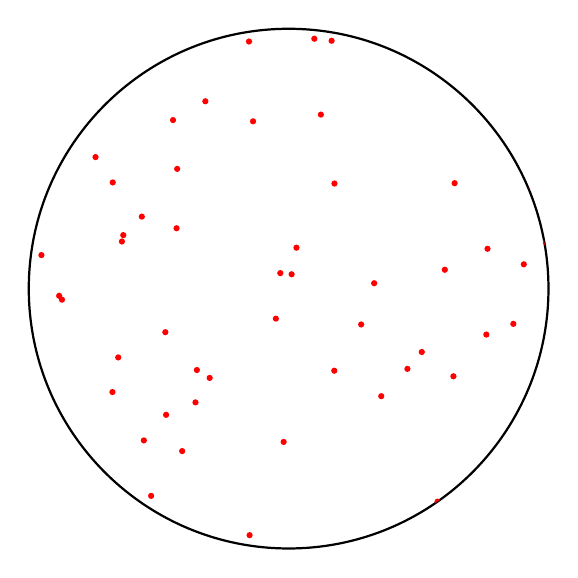
\begin{tikzpicture}[scale=0.22]
  \def\R{15}
  \draw[thick] (0,0) circle (\R);
  \begin{scope}
    \clip (0,0) circle (\R);
    \foreach \i in {1,...,60}{
      \pgfmathsetmacro{\xx}{(rnd*2-1)*\R}
      \pgfmathsetmacro{\yy}{(rnd*2-1)*\R}
      \fill[red] (\xx,\yy) circle (0.18);
    }
  \end{scope}
\end{tikzpicture}
\caption{Pause Refresh Fail のフェイルマップ例。
ロットを跨いでも同様のパターンが出現し,
プロセス条件起因であることが示唆された。}
\label{fig:failmap}
\end{figure}

\begin{figure}[t]
\centering
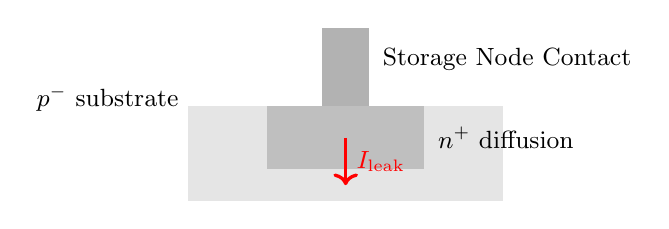
\begin{tikzpicture}[x=1cm,y=1cm]
  % p- substrate
  \fill[gray!20] (-2,0) rectangle (2,-1.2);
  \node[anchor=east] at (-2,0.1) {\small $p^-$ substrate};

  % n+ diffusion
  \fill[gray!50] (-1,0) rectangle (1,-0.8);
  \node[anchor=west] at (1.05,-0.4) {\small $n^+$ diffusion};

  % storage node contact
  \fill[black!30] (-0.3,0) rectangle (0.3,1.0);
  \node[anchor=west] at (0.35,0.6) {\small Storage Node Contact};

  % leakage arrow
  \draw[->,very thick,red] (0,-0.4) -- (0,-1.0)
    node[midway,right,red] {\small $I_{\mathrm{leak}}$};
\end{tikzpicture}
\caption{DRAMセル断面概念図。
SNコンタクト/n$^+$拡散層/p$^-$基板構造。
赤矢印は n$^+ \rightarrow p^-$ へのリーク電流 $I_{\mathrm{leak}}$ を示す。}
\label{fig:cell_leak}
\end{figure}

\subsection{プラズマダメージ仮説}
ジャンクションリーク増大の背景には,
\textbf{プラズマダメージ} が強く疑われた。  

具体的には以下の工程が影響源と考えられた:
\begin{itemize}
  \item ゲートエッチ後の酸化膜露出状態でのO$_2$プラズマ処理
  \item LDD形成工程での繰返しアッシング
\end{itemize}

O$_2$プラズマは酸化膜界面に欠陥準位を生成し,
熱励起キャリアのリークパスを形成する可能性がある。  
高温条件下でリーク電流が急増する挙動も観測されており,
プラズマ起因欠陥が主要因であるとの仮説を強める結果とだった。

\subsection{対策と効果}
根本対策は,
\textbf{「O$_2$アッシング剥離から硫酸ウェット剥離への全面切替」}であった。  
これによりプラズマ曝露を完全に排除し,
界面欠陥の生成を防ぐことに成功した。  

\begin{table}[h]
  \centering
  \caption{レジスト剥離フローの切替と効果}
  \label{tab:resist}
  \begin{tabular}{lll}
    \toprule
    & 従来 & 対策後 \\
    \midrule
    剥離方式 & O$_2$アッシング & 硫酸ウェット \\
    主効果 & 繰返しプラズマ曝露 & 界面欠陥防止 \\
    歩留まり & 約65\% & 80\%台後半へ改善 \\
    \bottomrule
  \end{tabular}
\end{table}

対策後,Pause不良は顕著に減少し,
歩留まりは安定して80\%台後半を示した
(Fig.~\ref{fig:yield25})。  

\begin{figure}[t]
\centering
\begin{tikzpicture}
\begin{axis}[
  width=\linewidth, height=6cm,
  ymin=0, ymax=100,
  ylabel={歩留まり (\%)},
  xtick={1,2,3,4},
  xticklabels={0.5um(16M),0.35um(64M),0.25um(64M),VSRAM},
  grid=both,
  legend style={
    at={(0.5,-0.25)},
    anchor=north,
    legend columns=-1,
    draw=none, fill=none
  }
]
  \addplot+[mark=*] coordinates {(1,95) (2,20) (3,65) (4,30)};
  \addlegendentry{初期}
  \addplot+[mark=square*] coordinates {(1,95) (2,86) (3,88) (4,80)};
  \addlegendentry{改善後}
\end{axis}
\end{tikzpicture}
\caption{酒田Fabにおける世代別歩留まり推移}
\label{fig:yield_all}
\end{figure}

\subsection{小括}
\begin{itemize}
  \item SCF方式により,従来を大きく上回る65\%の高い初期歩留まりを実現。
  \item 不良の主因はジャンクションリークであり,背後にはプラズマダメージが存在。
  \item O$_2$アッシングを硫酸ウェット剥離に置換することで,歩留まりは80\%台後半へと改善。
  \item 筆者は立ち上げ初期から参画し,プロセス解析・不良解析・量産対応を一貫して担当した。
\end{itemize}

\section{第3章:VSRAM(2001年)— Pause/Disturb対策と歩留まり改善}

\subsection{開発背景と初期状況}
2001年,当時の携帯電話市場は急速に進化しつつあった。
従来の音声端末から,カメラ・インターネット・マルチメディア機能を統合した
高性能端末への移行期であり,「世界初のカメラ付き携帯」の実現が各社の至上命題であった。  
その中で求められたのが,低消費電力かつ高温(90$^\circ$C)動作保証を備えたモバイル向けメモリであった。

酒田Fabは,\SI{0.25}{\micro\meter} DRAMプロセスを流用し,
内部リフレッシュ回路を付加した \emph{VSRAM(疑似SRAM)} を社内設計部門と連携して開発した。
モバイル市場を先行して獲得する戦略的狙いから,
初期量産歩留まりが約30\%に留まる状況でも,
「低歩留まりでも市場投入を優先する」という厳しい判断が下された。  
筆者はこの時点から改善担当として参画し,量産と並行して不良解析・対策を進める体制に入った。

\subsection{顕在化した不良モード}
VSRAMでは,従来のDRAMでは大きな問題とならなかった不良が,
モバイル環境特有の条件下で顕在化した。主な不良モードは以下の2種類である:
\begin{itemize}
  \item \textbf{Pause Refresh Fail}:リフレッシュ停止時にセル保持が崩壊する現象。
  \item \textbf{Disturb Refresh Fail}:隣接ワードラインの駆動による電圧干渉で誤反転が発生する現象。
\end{itemize}

PauseはDRAM固有の既知不良であったが,
Disturbは長リフレッシュ周期+高温動作というモバイル用途特有の条件で初めて顕在化した。

\subsection{物理的要因と解析プロセス}
Pause不良は,拡散層接合のリークに起因することが実験的に確証された。
保持時間モデル
\[
\tau = \frac{C_{\mathrm{cell}} V_{\mathrm{cell}}}{I_{\mathrm{leak}}}
\]
において,設計値 $C_{\mathrm{cell}}, V_{\mathrm{cell}}$ は規格内であるが,
リーク電流 $I_{\mathrm{leak}}$ の増大により $\tau$ が短縮していた。
温度を上げた評価では $I_{\mathrm{junc}}$ が指数関数的に増加し,
高温ほど保持特性が急激に劣化することが確認された(Fig.~\ref{fig:pause})。

一方 Disturb不良は,特定ワードラインに沿って系統的に発生することから,
短チャネル効果(SCE)が主因であることが特定された。
チャネル長が短いほど $I_{\mathrm{off}}$ が増大し,
高温動作でさらに顕著となった(Fig.~\ref{fig:disturb})。

% Fig. X  Pause Refresh:温度依存とバックバイアス効果(凡例は下中央)
\begin{figure}[t]
\centering
\begin{tikzpicture}
\begin{axis}[
  width=\linewidth, height=6cm,
  xlabel={温度 [$^\circ$C]}, ylabel={$I_{\mathrm{junc}}$ (相対)},
  ymode=log, ymin=1e-2, ymax=1e2,
  xmin=25, xmax=100, xtick={25,40,60,80,90,100},
  grid=both,
  legend style={
    at={(0.5,-0.25)}, anchor=north,
    legend columns=-1, draw=none, fill=none
  },
  clip=false
]
  % Vbs = -1 V
  \addplot+[semithick,mark=*] coordinates {
    (25,0.02) (40,0.06) (60,0.30) (80,1.60) (90,3.20) (100,6.00)
  };
  \addlegendentry{$V_{bs}=-1$ V}

  % Vbs = -3 V
  \addplot+[semithick,mark=square*] coordinates {
    (25,0.01) (40,0.03) (60,0.12) (80,0.45) (90,0.90) (100,1.80)
  };
  \addlegendentry{$V_{bs}=-3$ V}
\end{axis}
\end{tikzpicture}
\caption{Pause Refresh:ジャンクションリーク $I_{\mathrm{junc}}$ の温度依存。バックバイアス強化でリークが抑制される。}
\label{fig:pause_temp}
\end{figure}

% Fig. Y  Disturb Refresh:短チャネル効果と温度依存(凡例は下中央・"um"表記)
\begin{figure}[t]
\centering
\begin{tikzpicture}
\begin{axis}[
  width=\linewidth, height=6cm,
  xlabel={温度 [$^\circ$C]}, ylabel={$I_{\mathrm{off}}$ (相対)},
  ymode=log, ymin=1e-3, ymax=1e1,
  xmin=25, xmax=100, xtick={25,40,60,80,90,100},
  grid=both,
  legend style={
    at={(0.5,-0.25)}, anchor=north,
    legend columns=-1, draw=none, fill=none
  },
  clip=false
]
  % CD = 0.25 um
  \addplot+[semithick,mark=triangle*] coordinates {
    (25,0.004) (40,0.010) (60,0.050) (80,0.220) (90,0.450) (100,0.900)
  };
  \addlegendentry{CD = 0.25um}

  % CD = 0.20 um
  \addplot+[semithick,mark=*] coordinates {
    (25,0.010) (40,0.030) (60,0.150) (80,0.700) (90,1.400) (100,2.800)
  };
  \addlegendentry{CD = 0.20um}
\end{axis}
\end{tikzpicture}
\caption{Disturb Refresh:トランジスタ $I_{\mathrm{off}}$ の温度依存。チャネル長が短いほど(CD小)リークが急増する。}
\label{fig:disturb_temp}
\end{figure}

\subsection{対策と実装}
不良要因を踏まえ,以下の対策が実装された:
\begin{itemize}
  \item Pause対策:
    \begin{itemize}
      \item HF洗浄回数を最小化し,SNコンタクトリークを抑制。
      \item バックバイアスを $-1$V $\rightarrow$ $-3$V に強化し,ジャンクションリークを低減。
    \end{itemize}
  \item Disturb対策:
    \begin{itemize}
      \item ゲートCD管理を徹底し,設計通りのしきい値特性を確保。
      \item バックバイアス強化により $V_{th}$ を上昇させ,セル反転耐性を確保。
      \item チャネルドーピングを増加させ,短チャネル効果を抑制。
    \end{itemize}
\end{itemize}

これらの改善は設計・プロセス・製造の三部門横断で行われ,
試作評価と量産条件調整を同時並行で進める「走りながら直す」体制が敷かれた。

\subsection{改善効果と事業的インパクト}
Pause/Disturb不良は大幅に減少し,
歩留まりは初期30\%から半年以内に80\%台へ改善した。
この結果,酒田Fabは競合に先行してモバイルメモリを安定供給できる体制を確立した。  

市場的にも本製品は「世界初のカメラ付き携帯」に搭載され,
酒田Fabがモバイル市場に直接貢献した数少ない事例となった。
本改善活動は,\emph{酒田FabにおけるDRAM派生メモリ開発の集大成}と位置づけられる。

\subsection{小括}
\begin{itemize}
  \item モバイル市場先行投入を優先し,低歩留まりでも量産開始というリスクを取った。
  \item Pause/Disturbは高温動作・長リフレッシュ条件で顕在化し,リークと短チャネル効果が主因と特定された。
  \item HF洗浄制御,バックバイアス強化,ゲート寸法管理により歩留まりは30\%から80\%台へ改善。
  \item この成功は,酒田Fabがモバイル市場に対応可能であることを社内外に示し,
        DRAM派生メモリ開発の最終的成果となった。
\end{itemize}

\section{第4章:\texorpdfstring{\SI{0.18}{\micro\meter}}{0.18µm} トレンチ系の評価と断念}

\subsection{評価対象と背景}
2001年のVSRAM量産立ち上げ後,酒田Fabでは次世代モバイルメモリの開発が検討された。  
候補の一つが,台湾NANYA社の \SI{0.18}{\micro\meter} DRAMプロセスを利用したVSRAMである。  
NANYAは東芝と技術提携を行っており,その技術は \emph{トレンチキャパシタ方式} を基盤としていた。  

目的は,既存の \SI{0.25}{\micro\meter} DRAM流用VSRAMを凌駕し,  
さらなる高密度化,低消費電力化,および高温(90$^\circ$C)動作保証を満たす次世代モバイル向けメモリを確立することであった。

\subsection{技術的特徴}
本評価プロセスには以下の特徴があった:
\begin{itemize}
  \item \textbf{キャパシタ構造}:従来のスタック型に比べ,面積効率の高いトレンチ型を採用。  
        セル面積の縮小が可能であり,高密度化に優位。
  \item \textbf{動作仕様}:標準DRAMと同様に80$^\circ$Cでの動作保証は可能であったが,  
        モバイル用途に必須の90$^\circ$C保証には大きな課題を抱えていた。
\end{itemize}

\subsection{課題の顕在化}
試作評価の結果,90$^\circ$C条件下で以下の不良が顕著に現れた:
\begin{itemize}
  \item \textbf{Pause Refresh Fail}:セル保持時間が不足し,動作マージンが消失。
  \item \textbf{Disturb Refresh Fail}:高温条件下で隣接ワードライン干渉による誤反転が多発。
  \item \textbf{高温リーク}:pn接合リークが顕著に増加し,セル保持特性を支配。
\end{itemize}

\subsection{構造的起因の解析}
Fig.~\ref{fig:stack_trench} に示すように,  
Stack型では接合が拡散層の側壁と底面に限定され,周辺長は比較的短い。  
一方,Trench型ではセルごとに \emph{buried strap} 接続部を介して局所接合が形成され,  
セル列の繰り返し構造により実質的な周辺長が大幅に増加する。  

この構造差により,ジャンクションリークの起点が増加し,  
高温条件でのリーク電流は指数的に増大した(Fig.~\ref{fig:trench_leak})。  

% ==== Fig. Stack vs. Trench:断面と上面(1カラム) ====
\begin{figure}[t]
\centering

% -------- Group title: Cross-sections --------
\textit{Cross-sections}\par\vspace{0.3em}

% (a) Stack Cross-section  — 縦
\subfloat[(a) Stack Cross-section]{%
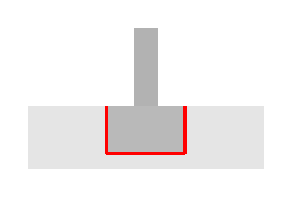
\begin{tikzpicture}[x=1cm,y=1cm]
  % p- substrate
  \fill[gray!20] (-1.5,0) rectangle (1.5,-0.8);
  % n+ diffusion
  \fill[gray!55] (-0.5,0) rectangle (0.5,-0.6);
  % storage node
  \fill[black!30] (-0.15,0) rectangle (0.15,1.0);
  % pn junction perimeter (red)
  \draw[red,very thick] (-0.5,0) -- (-0.5,-0.6);
  \draw[red,very thick] ( 0.5,0) -- ( 0.5,-0.6);
  \draw[red,very thick] (-0.5,-0.6) -- (0.5,-0.6);
\end{tikzpicture}
\label{fig:stack_trench_a}}
\par\vspace{0.6em}

% (b) Trench Cross-section — 縦
\subfloat[(b) Trench Cross-section]{%
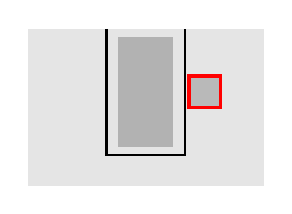
\begin{tikzpicture}[x=1cm,y=1cm]
  % p- substrate
  \fill[gray!20] (-1.5,0) rectangle (1.5,-2.0);
  % trench cavity
  \draw[black,thick] (-0.5,0) -- (-0.5,-1.6) -- (0.5,-1.6) -- (0.5,0);
  % trench electrode
  \fill[black!30] (-0.35,-0.1) rectangle (0.35,-1.5);
  % buried strap diffusion
  \fill[gray!55] (0.55,-0.6) rectangle (0.95,-1.0);
  % pn junction highlight
  \draw[red,very thick] (0.55,-0.6) rectangle (0.95,-1.0);
\end{tikzpicture}
\label{fig:stack_trench_b}}
\par\vspace{0.9em}

% -------- Group title: Top views --------
\textit{Top views}\par\vspace{0.3em}

% (c) Stack Top view  — 左
\subfloat[(c) Stack Top view]{%
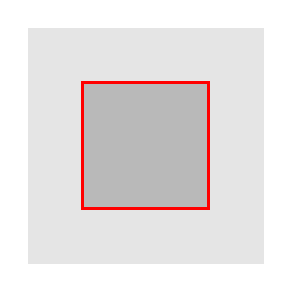
\begin{tikzpicture}[x=1cm,y=1cm]
  % p- substrate(残す)
  \fill[gray!20] (-1.5,-1.5) rectangle (1.5,1.5);
  % n+ diffusion area
  \fill[gray!55] (-0.8,-0.8) rectangle (0.8,0.8);
  % ※中央の薄い四角は入れない(指摘反映)
  % pn junction perimeter
  \draw[red,very thick] (-0.8,-0.8) rectangle (0.8,0.8);
\end{tikzpicture}
\label{fig:stack_trench_c}}
\hfill
% (d) Trench Top view  — 右(修正)
\subfloat[(d) Trench Top view]{%
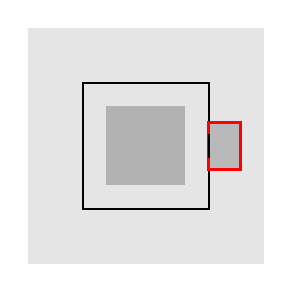
\begin{tikzpicture}[x=1cm,y=1cm]
  % p- substrate(残す)
  \fill[gray!20] (-1.5,-1.5) rectangle (1.5,1.5);
  % trench cavity(開口)
  \draw[black,thick] (-0.8,-0.8) rectangle (0.8,0.8);
  % trench electrode(内部電極)
  \fill[black!30] (-0.5,-0.5) rectangle (0.5,0.5);
  % buried strap(壁に接した接続拡散。位置を修正)
  \fill[gray!55] (0.80,-0.30) rectangle (1.20,0.30);
  % pn junction highlight(strap 周囲を赤枠で強調)
  \draw[red,very thick] (0.80,-0.30) rectangle (1.20,0.30);
  % 視覚的な“接続”を示す短いブリッジ(任意)
  \draw[black,thick] (0.80,-0.15) -- (0.80,0.15);
\end{tikzpicture}
\label{fig:stack_trench_d}}

\caption{Stack と Trench キャパシタ構造の比較:断面(a,b)および上面(c,d)。  
Stack は接合周辺長が限定的であるのに対し,Trench は \textit{buried strap} 起点で周辺長が増大し,高温リークのリスクが高い。}
\label{fig:stack_trench}
\end{figure}

\begin{figure}[t]
\centering
\begin{tikzpicture}
\begin{axis}[
  width=\linewidth, height=6cm,
  xlabel={ジャンクション面積(相対)}, ylabel={$I_{\mathrm{junc}}$(相対)},
  xmin=0.5, xmax=2.5, ymin=0, ymax=3,
  grid=both,
  legend style={at={(0.5,-0.22)},anchor=north,draw=none,fill=none},
  clip=false
]
  \addplot+[mark=square*] coordinates {
    (0.5,0.25) (1.0,0.5) (1.5,0.8) (2.0,1.1) (2.5,1.4)
  };
  \addlegendentry{80$^\circ$C}
  \addplot+[mark=*] coordinates {
    (0.5,0.5) (1.0,1.0) (1.5,1.6) (2.0,2.2) (2.5,2.9)
  };
  \addlegendentry{90$^\circ$C}
\end{axis}
\end{tikzpicture}
\caption{トレンチ型セルにおけるジャンクションリークの面積依存性。
高温条件では増加率がさらに顕著である。}
\label{fig:trench_leak}
\end{figure}

\subsection{評価結果と戦略判断}
総合評価の結果,NANYA \SI{0.18}{\micro\meter} トレンチプロセスは
モバイル用途に必須の90$^\circ$C動作保証を満たすことができず,
次世代VSRAMとしては不適であると判断された。  

この判断により,酒田FabでのDRAM派生製品開発は終息へと向かい,  
経営資源は液晶ドライバー向けの高耐圧混載CMOS開発に集中する方針が固まった。  

\subsection{小括}
\begin{itemize}
  \item トレンチ方式は高密度化には有利だが,高温リーク増大でモバイル仕様に適さなかった。
  \item 90$^\circ$C保証を満たせず,次世代VSRAMは断念。
  \item 以後は液晶ドライバーを中心とする高耐圧混載CMOS開発へと戦略転換した。
\end{itemize}

\section{結論}

本研究では,1997年から2001年にかけて酒田Fabで行われた
DRAM技術導入と量産化の過程を,筆者の現場経験に基づいて整理した。

\begin{itemize}
  \item \textbf{第1章}:\SI{0.5}{\micro\meter} 世代16M DRAMは熊本Fabプロセスの忠実移管で安定立ち上げ。
        \SI{0.35}{\micro\meter} 世代64M DRAMでは洗浄フロー差異が原因で大規模不良が発生したが,
        熊本条件の完全「鏡写し」によって解決し,移管プロセスにおける
        「二次因子も含めて省略不可」という教訓がFab全体に共有された。
  \item \textbf{第2章}:\SI{0.25}{\micro\meter} 世代64M DRAMはSCF方式により短期間で立ち上げ。
        初期歩留まり65\%からスタートし,不良解析でジャンクションリークを主因と特定。
        O$_2$アッシングを硫酸ウェット剥離に切り替えることで,
        歩留まりは80\%台後半に改善した。
  \item \textbf{第3章}:VSRAMではモバイル要求(低消費・90$^\circ$C保証)がPause/Disturb不良を顕在化させた。
        HF洗浄回数の最小化,バックバイアス強化,ゲート寸法管理などにより,
        歩留まりは30\%から80\%台へ改善。酒田FabにおけるDRAM派生メモリ開発の集大成となった。
  \item \textbf{第4章}:NANYA \SI{0.18}{\micro\meter} トレンチプロセスの評価では,
        高温リークの増大により90$^\circ$C保証を満たせず,次世代VSRAMは断念。
        これにより酒田Fabでのメモリ派生製品開発は終息に向かい,
        経営資源は液晶ドライバー向け高耐圧混載CMOSに集中した。
\end{itemize}

\noindent
総括すると,酒田FabにおけるDRAM導入は,
DRAMそのものを事業の柱とする狙いではなく,
\textbf{最新世代の装置・プロセス・量産立ち上げ能力を獲得するための手段}であった。  

DRAM量産ラインを通じて確立されたインフラは,
\begin{itemize}
  \item 外販ファンドリ(Xilinx等)との協働による先端ロジックプロセス,
  \item 社内ロジックSoC/マイコン開発,
  \item 液晶ドライバーを中心とする高耐圧混載CMOS
\end{itemize}
といった複線的な事業展開を可能にした。これらはそれぞれ専任部隊により推進されたものであり,
DRAM不良対策の知見が直接移植されたわけではない。  

\noindent
すなわち,DRAMおよびVSRAMは最終的に事業としては終息したが,
その導入がエプソンにとっての「戦略的成功」であったことに疑いはない。  
DRAMを通じて整備された量産インフラは,
先端ロジック,社内SoC/マイコン,高耐圧混載CMOSによる液晶ドライバー事業といった
後続ビジネスの基盤を支え,エプソンの半導体戦略の中核を形成した。

\section*{参考文献}
\begin{thebibliography}{00}
\bibitem{sze2006psd}
S.~M.~Sze and K.~K.~Ng, \emph{Physics of Semiconductor Devices}, 3rd ed., Wiley, 2006.

\bibitem{tanaka1996dramtrends}
T.~Tanaka et al., ``Trends and Challenges in DRAM Scaling,'' \emph{IEEE J. Solid-State Circuits}, vol.~31, no.~11, pp.~1615--1624, 1996.

\bibitem{rizzoli2000retention}
L.~Rizzoli et al., ``Retention and Disturb Characterization in 0.25 Micron DRAM,'' in \emph{Proc. Int. Test Conf.}, 2000.

\bibitem{okhonin1998retention}
S.~Okhonin et al., ``Retention Time and Junction Leakage in Deep Submicron DRAM,'' in \emph{IEDM Tech. Dig.}, pp.~549--552, 1998.

\bibitem{wong1999dram}
H.-S.~P.~Wong, ``Technology and Device Scaling for DRAM,'' \emph{IBM J. Res. Dev.}, vol.~43, no.~1–2, pp.~133--168, 1999.

\bibitem{chang1994plasma}
C.~Chang and S.~C.~Lee, ``Plasma-Induced Damage on Gate Oxides,'' \emph{J. Electrochem. Soc.}, vol.~141, no.~9, pp.~2512--2517, 1994.

\bibitem{mosys2001}
MoSys Inc., ``1T-SRAM Technology Overview,'' White Paper, 2001.

\bibitem{kim2002psram}
J.~Kim et al., ``Low Power Refresh Schemes for Mobile DRAM/PSRAM,'' in \emph{Symp. on VLSI Circuits}, pp.~190--193, 2002.

\bibitem{schuegraf1997plasma}
K.~Schuegraf et al., ``Impact of Plasma Damage on Junction Leakage and Gate Oxide Reliability,'' in \emph{VMIC Conf. Proc.}, pp.~73--79, 1997.
\end{thebibliography}

\section*{著者略歴}
\noindent\textbf{三溝 真一 (Shinichi Samizo)}  
信州大学大学院 工学系研究科 電気電子工学専攻修士課程を修了後,
セイコーエプソン株式会社に勤務。  
半導体ロジック/メモリ/高耐圧インテグレーション,
インクジェット薄膜ピエゾアクチュエータ,
および PrecisionCore プリントヘッドの製品化に従事した。  
現在は独立系半導体研究者として,
プロセス/デバイス教育,メモリアーキテクチャ,AIシステム統合に取り組んでいる。  
連絡先: \href{mailto:shin3t72@gmail.com}{shin3t72@gmail.com}

\end{document}
